
%%%%%%%%%%%%%%%%%%%%%%%%%%%%%%%%%%%%%%%%%%%%%%%%%%%%%%%%%%%%%%%%%%%%%
%% PREAMBLE
%%%%%%%%%%%%%%%%%%%%%%%%%%%%%%%%%%%%%%%%%%%%%%%%%%%%%%%%%%%%%%%%%%%%%
%
% The following two commands will generate a PDF that follows all the requirements for submission
% and peer review.  Uncomment these commands to generate this output (and comment out the two lines below.)
%
% DOUBLE SPACE VERSION FOR SUBMISSION TO THE AMS2

\documentclass[12pt,varwidth]{article}
\usepackage{ametsoc}
%\usepackage{ametsoc2col}
\usepackage{graphicx}
\usepackage{amsmath}
\usepackage{amssymb}
\usepackage{subfig}
\usepackage{setspace}
\usepackage[%
  color=gray
 ,scale=8
]{background}

\backgroundsetup{contents={DRAFT}}
%\usepackage[mathlines]{lineno} 
%
% The following two commands will generate a single space, double column paper that closely
% matches an AMS journal page.  Uncomment these commands to generate this output (and comment
% out the two lines above. FOR AUTHOR USE ONLY. PAPERS SUBMITTED IN THIS FORMAT WILL BE RETURNED
% TO THE AUTHOR for submission with the correct formatting.
%
% TWO COLUMN JOURNAL PAGE LAYOUT FOR AUTHOR USE ONLY
%%%%\documentclass[10pt]{article}
%%%%\usepackage{ametsoc2col}
% new commands
\newcommand{\xmathbf}{\boldsymbol}
\def\cam{CAM4}
\def\deg{$^\circ$}
%
%%%%%%%%%%%%%%%%%%%%%%%%%%%%%%%%%%%%%%%%%%%%%%%%%%%%%%%%%%%%%%%%%%%%%
% ABSTRACT
%
% Enter your Abstract here
%%%%%%%%%%%%%%%%%%%%%%%%%%%%%%%%%%%%%%%%%%%%%%%%%%%%%%%%%%%%%%%%%%%%

\newcommand{\myabstract}{Atmospheric blocking is a major mode of sub-seasonal variability in the northern hemisphere. It has historically been a challenge for forecast and climate models alike and remains so. Blocking events are central to extreme Summer-time and Winter-time weather and as such are key to understanding impacts in a week's time and in a future warmer world. We show the evolution of atmospheric blocking in AMIP-type simulations between CAM3 and CAM5. Winter-time event frequency is 50\% or less of the observed blocking in the north Atlantic. This is only marginally improved between model versions. In contrast Spring-time and Summer-time blocking frequency improves monotonically between model versions, particularly in the North Atlantic. Significant sensitivities exist related to horizontal and vertical resolution, dynamical core and physics. Improvements in North Atlantic blocking are clearly related to improvements in the local jet characteristics. Somewhat surprisingly event duration distributions are well captured in all model versions, implying that blocking differences are largely related to mean climate changes.

Investigation of the reasons for the improvements in blocking between CAM3 and CAM5 shows that the key physics changes were the inclusion of deep convection parcel dilution in CAM4 and the turbulent mountain stress in CAM5. The change of dynamical from global spectral to finite volume results in a degradation of the simulation whereas the use of a spectral element core has little impact on the simulation.
-Dycore dependence varies with season.
-Eul actually best
-Loss of skill CAM3->CAM4 is in large part due to dy-core change in DJF. Not so much other seasons.
-FV/SE equivalent
-High-res SE poorer


}

\begin{document}

%
%%%%%%%%%%%%%%%%%%%%%%%%%%%%%%%%%%%%%%%%%%%%%%%%%%%%%%%%%%%%%%%%%%%%%
% TITLE
%
% Enter your TITLE here
%%%%%%%%%%%%%%%%%%%%%%%%%%%%%%%%%%%%%%%%%%%%%%%%%%%%%%%%%%%%%%%%%%%%%
\title{\textbf{\large{Evolution of Blocking Metrics and Mean Climate in Multiple Versions of the Community Atmosphere Model (CAM)}}}
%
% Author names, with corresponding author information. 
% [Update and move the \thanks{..} block as appropriate.]
%
\author{\textsc{Richard B. Neale}
				\thanks{\textit{Corresponding author address:} 
				Dr. Richard B. Neale, National Center for Atmospheric Research, 
				P.O. Box 3000, Boulder, CO 80307. 
				\newline{E-mail: rneale@ucar.edu}},\quad\textsc{Cecile Hannay}, \\  and\quad\textsc{Jadwiga Richter}\\
\textit{\footnotesize{National Center for Atmospheric Research, Boulder Colorado}}
}
%
% Formatting done here...Authors should skip over this.  See above for abstract.
\ifthenelse{\boolean{dc}}
{
\twocolumn[
\begin{@twocolumnfalse}
\amstitle

% Start Abstract (Enter your Abstract above.  Do not enter any text here)
\begin{center}
\begin{minipage}{13.0cm}
\begin{abstract}
	\myabstract
	\newpage
	\begin{center}
		\rule{38mm}{0.2mm}
	\end{center}
\end{abstract}
\end{minipage}
\end{center}
\end{@twocolumnfalse}
]
}
{
\amstitle
\linenumbers
\begin{abstract}
\myabstract
\end{abstract}
}
\newpage
%%%%%%%%%%%%%%%%%%%%%%%%%%%%%%%%%%%%%%%%%%%%%%%%%%%%%%%%%%%%%%%%%%%%%
% MAIN BODY OF PAPER
%%%%%%%%%%%%%%%%%%%%%%%%%%%%%%%%%%%%%%%%%%%%%%%%%%%%%%%%%%%%%%%%%%%%%
\section{Introduction}

Additional plots:
-EKE x-axis, vs blocking y-axis
-1d and 2d variance of blocking
-Variations of blocking (1D) with physics settings
-A quick plot of Greenland removal/X2 changes?
-Blocking with the removal of the basic state?
-NAO vs. blocking relationships?
-




Atmospheric blocking is a major mode of variability in the mid-latitude Northern Hemisphere \citep{Rex50} on synoptic to intra-seasonal timescales. It predominantly exists as a slower, quasi-stationary mode of variability compare the more frequent mid-latitude baroclinic activity. The asynoptic, persistent phenomena are often associated with extreme weather events either locally or remotely from the blocking centers. This can include anomalously cold temperatures in Summer and warm temperatures in winter. The persistent nature of blocking is the key factor in determining the impact of blocking. In summer, one or two days of extreme temperatures cab be tolerated but many days in a row often leads to the largest observed impact. The European summer heat wave of 2003

Different measures of blocking based on 500-mb height fields potential vorticity analysis and cite \citep{Barnes12} with multiple  

What causes blocking. Winter and summer.

Seasonal influences on blocking have been shown for El Nino, La Nina

Global climate models (GCMs) have been shown to under perform in simulating various characteristics of blocking events \citep{Mosato13}. In particular wintertime Euro-Atlantic blocking frequency is significantly underestimated in most CMIP3 and CMIP5 \citep{Dunn13} models wheres North Pacific frequency is reduced.

Reasons for limitations in blocking including basic state biases \citep{Scaife10}

The poor performance in models over the observational period reduces confidence in how blocking may change in the future and more importantly how associated extreme temperature and precipitation event statistics may change. 

Understanding the role of different aspects of GCM configurations such as choice of physical parameterization, dynamical core, grid resolution and surface couping has proven difficult such that addressing blocking shortcomings in response to these factors has proven challenge, mostly because the processes that lead to blocking remain uncertain? Future winter-time blocking event length has been shown to remain approximately constant in CMIP3 models, but frequency is largely reduced \citep{Barnes12}.

Centers of maximum blocking activity are located in the Atlantic and Pacific ocean basins.
-Characterization (Rex et al)
-Atlantic/Pacific/DJF/MAM maxima
-Role of basic state
-Importance for extreme events


Influence of tropical atlantic \cite{Cassou05}
Cassou et al (2005)
-Pakistan flooding due to 2010 Russia heatwave \cite{Galarneau12}


In this paper we examine the performance of the a suite of Community Atmosphere Model simulations in simulating multiple characteristics of blocking phenomenon. In section 2 we outline the model versions and simulations used and then contrast their mean climate differences. Blocking behavior using standard metrics and diagnostics in section 4. Section 5 examines composite geographic blocking patterns and section 6 identifies the specific model differences that distinguish CAM blocking behavior. We presents conclusions in Section 5 


\section{Models and Experiments}

The Community Atmosphere Model (CAM) is the atmospheric component of the Community Earth System Model (CESM). In this paper we examine the evolution of CAM development over three model versions. CAM3 \citep{CAM3}, CAM4 \citep{CAM4} and CAM5 \citep{CESM1}. The model versions exhibit a significant evolution in the representations of the moist physics, progressively improving many aspects of their simulations. CAM

\section{Climate Differences}
The evolution of climate simulations using CAM3 through CAM5 model versions are well documented are well documented \citep{CAM3,CCSM3,CAM4,CCSM4_oview,CESM1}

\section{Blocking Performance}
A number of modifications have been implemented in CAM4, the most impactful of which are summarized below. A more comprehensive description of CAM4 can be found in \citet{CAM4_TN}.

\subsection{Blocking Indices}
We first diagnose the simulation of blocking in CAM in terms of event frequency. 
\subsubsection{Frequency}
\subsection{Annual Cycle}
\subsubsection{Strength}

\subsection{Period Length}

A key measure of blocking in terms of the impact on extreme weather is the persistence of individual event. Even though daily blocking frequency may have been simulated accurately in CAM that does not necessarily speak to the correct distribution of event length. The the impact in terms of extreme weather is much more profound for a single blocking event that lasts 10 days versus 10 single-day events. Fig \

\subsection{Composite Events}
Knowing the distribution of blocking and baroclinic strength as shown in \label{} we are able to evaluate composite events based on the an average of the top (blocked) and bottom (baroclinic) 10\% Z500 strength days for each mean blocking maximum region (European and Pacific blocking centers).In Winter all model versions are able to capture the Western zonal extent of the composite Z500 block pattern, this is despite getting the frequency of these blocking events correct. The models correctly reproduce associated l

-Remember these composites only show what the top/bottom percentile events look like not they are stronger or occur more frequently in CAM5/MAM for example. But maybe one would expect CAM5 in winter to have a stronger spring pattern?

-Both baroclinic and barotropic composite anomalies are of equal strength at zero lag, but blocking anomalies remain much larger at -/+ 5 days indicating the longer persistence of blocking events in both observations and all versions of CAM.

-In CAM the blocking centers seem to grow and decay in-situ over the European region five days prior to and following the lag-zero blocking. This is in contrast to ERAI where the blocking center is located in the central Atlantic five days prior to the zero lag day and then decays in-situ north of the UK.

-REMEMBER: Blocking improves in MAM, not so much in DJF, so there should not really be an expectation of differences in DJF really.

-In DJF the strongest circulation features over the USA are seen with a lag of -3 days. This is not 


\section{Conclusions}


\begin{acknowledgment} 
Support of this research project.
\end{acknowledgment}


\nolinenumbers
% Use appendix}[A], {appendix}[B], etc. etc. in place of appendix if you have multiple appendixes.
%\ifthenelse{\boolean{dc}}
{}
{\clearpage}
%\begin{appendix}
%\section*{\begin{center}Appendix Title Is Entered Here (Primary heading)\end{center}}
%\subsection{First appendix secondary heading}

%\subsection{Second appendix secondary heading}

%\subsubsection{First appendix tertiary heading}

%\subsubsection{Second appendix tertiary heading}

%\paragraph{First appendix quarternary heading}

%\paragraph{Second appendix quarternary heading}

%\end{appendix}

% Create a bibliography directory and place your .bib file there.
\ifthenelse{\boolean{dc}}
{}
{\clearpage}
\bibliographystyle{./ametsoc}
\bibliography{./references}
\pagebreak

%%%%%%%%%%%%%%%%%%%%%%%%%%%%%%%%%%%%%%%%%%%%%%%%%%%%%%%%%%%%%%%%%%%%%
% FIGURES
%%%%%%%%%%%%%%%%%%%%%%%%%%%%%%%%%%%%%%%%%%%%%%%%%%%%%%%%%%%%%%%%%%%%%

\begin{figure}[t]
  \begin{center}
    \noindent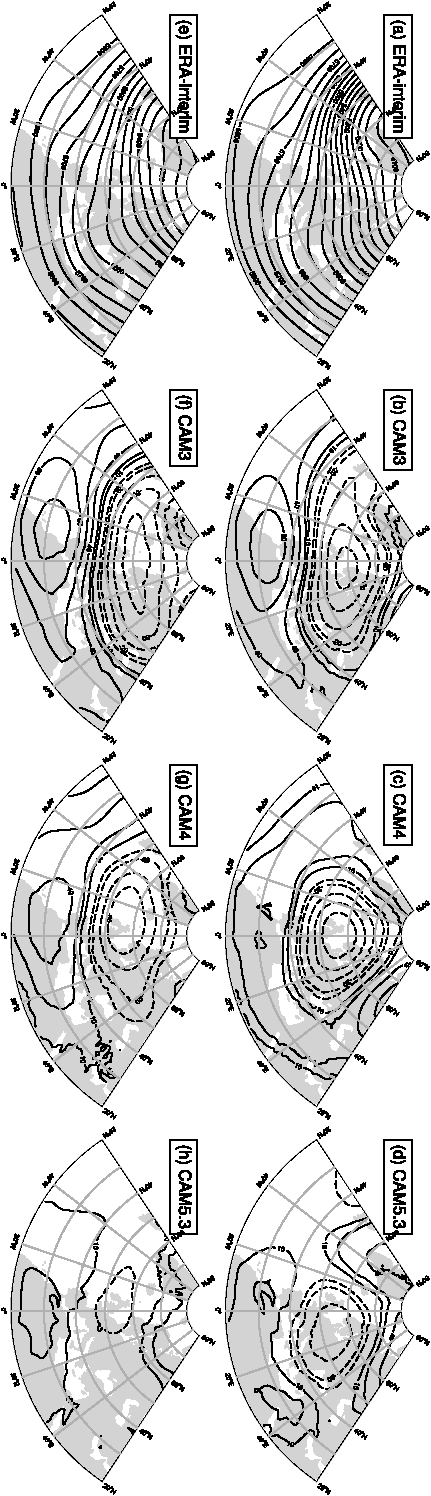
\includegraphics[width=0.3\textwidth,angle=90.]{./figs/f_mean_Z500_atl.pdf}\\
  \end{center}
  \caption{500-hPa height (m) over the Atlantic sector during Dec/Jan/Feb (top) and Mar/Apr/May (bottom) for ERA-interim (a,e) and seasonal biases in the ensemble average of CAM3 (b,f), CAM4 (c,g) and CAM5 (d,h) simulations}
\label{f_mean_Z500_atl}
\end{figure}

\begin{figure}[t]
  \begin{center}
    \noindent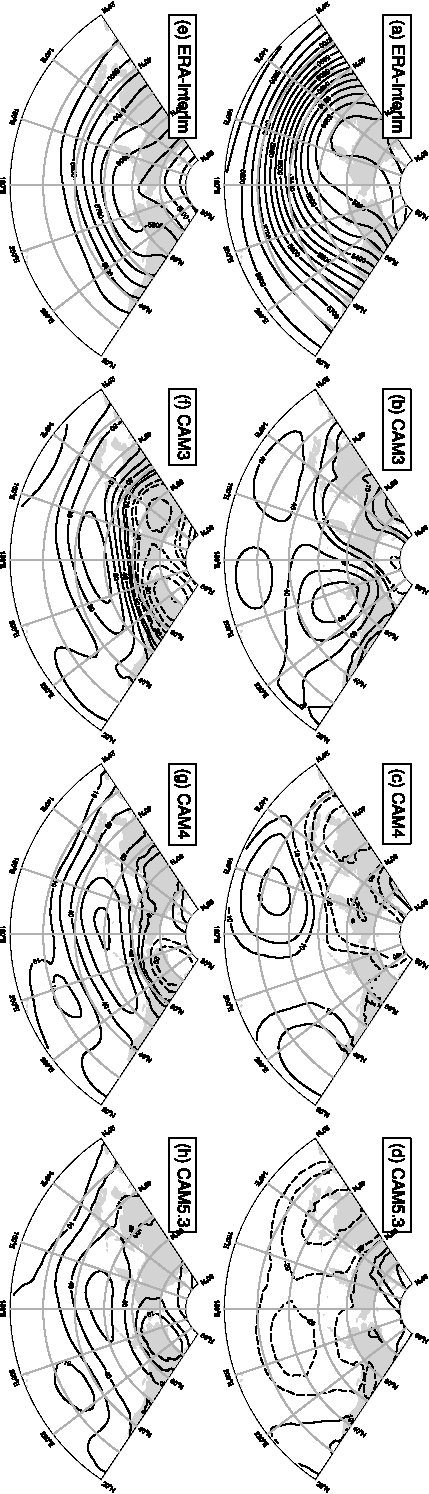
\includegraphics[width=0.3\textwidth,angle=90.]{./figs/f_mean_Z500_pac.pdf}\\
  \end{center}
  \caption{500-hPa height (m) over the Pacific sector during Dec/Jan/Feb (top) and Mar/Apr/May (bottom) for ERA-interim (a,e) and seasonal biases in the ensemble average of CAM3 (b,f), CAM4 (c,g) and CAM5 (d,h) simulations}
\label{f_mean_Z500_pac}
\end{figure}

\begin{figure}[t]
  \begin{center}
    \noindent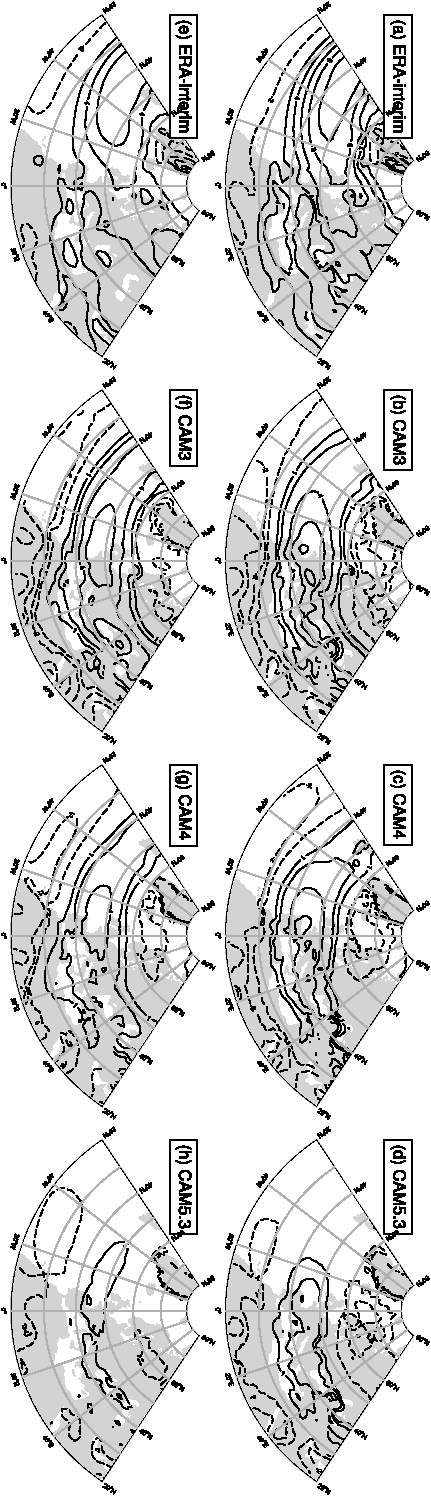
\includegraphics[width=0.3\textwidth,angle=90.]{./figs/f_mean_U850_atl.pdf}\\
  \end{center}
  \caption{850-hPa zonal wind (ms$^{-1}$) over the Atlantic sector during Dec/Jan/Feb (top) and Mar/Apr/May (bottom) for ERA-interim (a,e) and seasonal biases in the ensemble average of CAM3 (b,f), CAM4 (c,g) and CAM5 (d,h) simulations}
\label{f_mean_U850_atl}
\end{figure}

\begin{figure}[t]
  \begin{center}
    \noindent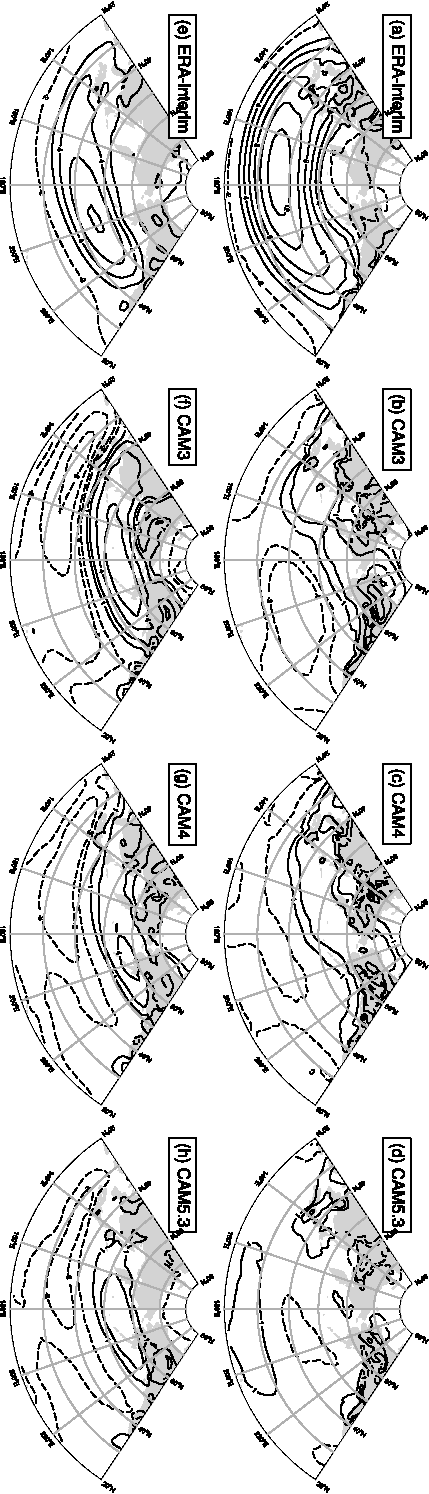
\includegraphics[width=0.3\textwidth,angle=90.]{./figs/f_mean_U850_pac.pdf}\\
  \end{center}
  \caption{850-hPa zonal wind (ms$^{-1}$) over the Pacific sector during Dec/Jan/Feb (top) and Mar/Apr/May (bottom) for ERA-interim (a,e) and seasonal biases in the ensemble average of CAM3 (b,f), CAM4 (c,g) and CAM5 (d,h) simulations}
\label{f_mean_U850_pac}
\end{figure}

\begin{figure}[t]
  \begin{center}
    \noindent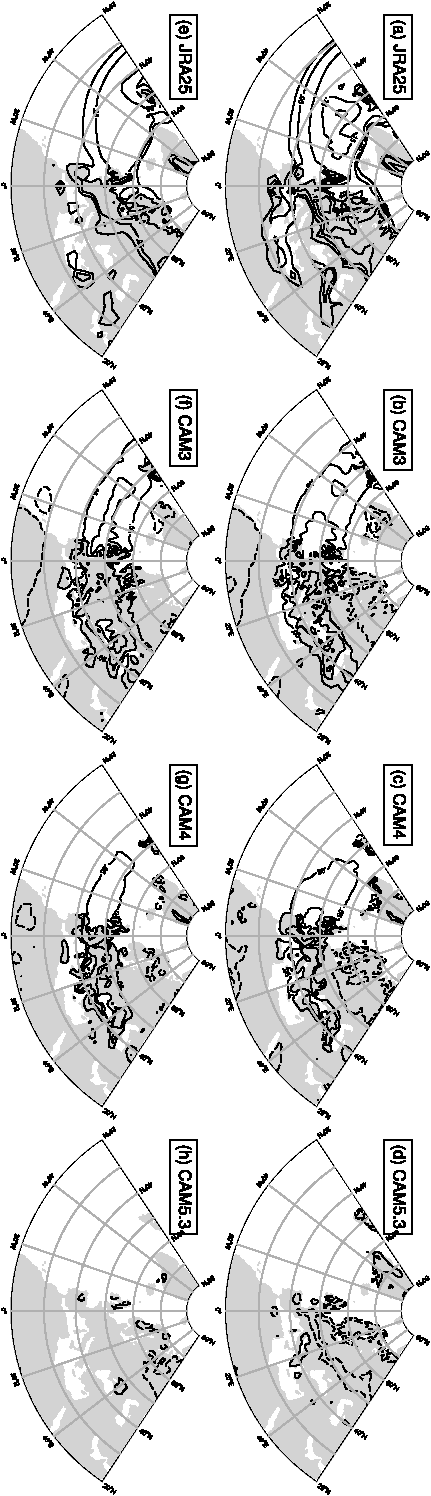
\includegraphics[width=0.3\textwidth,angle=90.]{./figs/f_mean_TAUX_atl.pdf}\\
  \end{center}
  \caption{Surface zonal stress (Nm$^{-2}$) over the Atlantic sector during Dec/Jan/Feb (top) and Mar/Apr/May (bottom) for JRA25 (a,e) and seasonal biases in the ensemble average of CAM3 (b,f), CAM4 (c,g) and CAM5 (d,h) simulations}
\label{f_mean_TAUX_atl}
\end{figure}

\begin{figure}[t]
  \begin{center}
    \noindent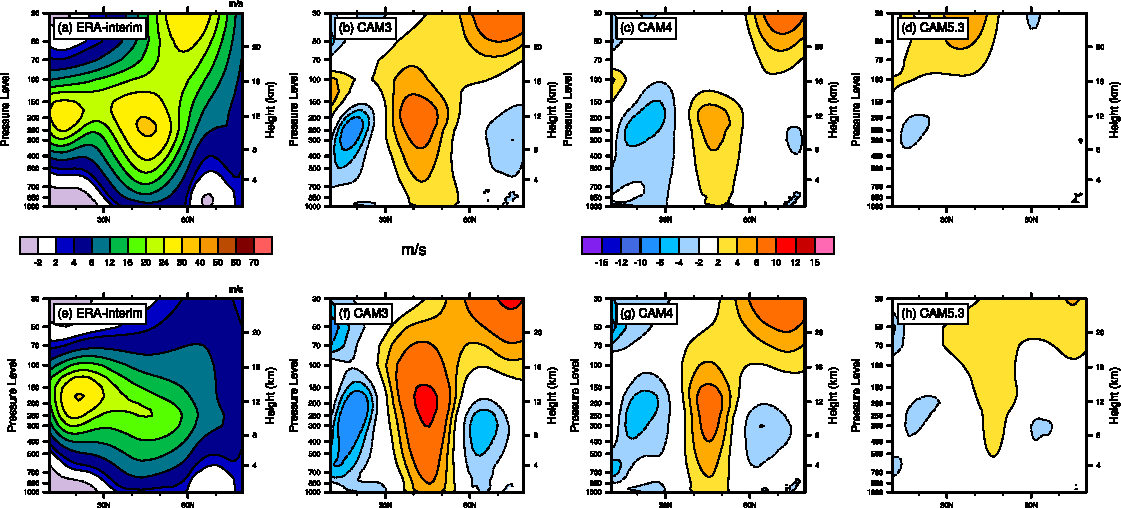
\includegraphics[width=1.0\textwidth,angle=0.]{./figs/f_U_atl.pdf}\\
  \end{center}
  \caption{Zonal wind (ms$^{-1}$) over the Atlantic sector (60\deg W-20\deg W) from ERA-interim (a,e) and seasonal biases in the ensemble average of CAM3 (b,f), CAM4 (c,g) and CAM5 (d,h) simulations}
\label{f_U_atl}
\end{figure}

\begin{figure}[t]
  \begin{center}
    \noindent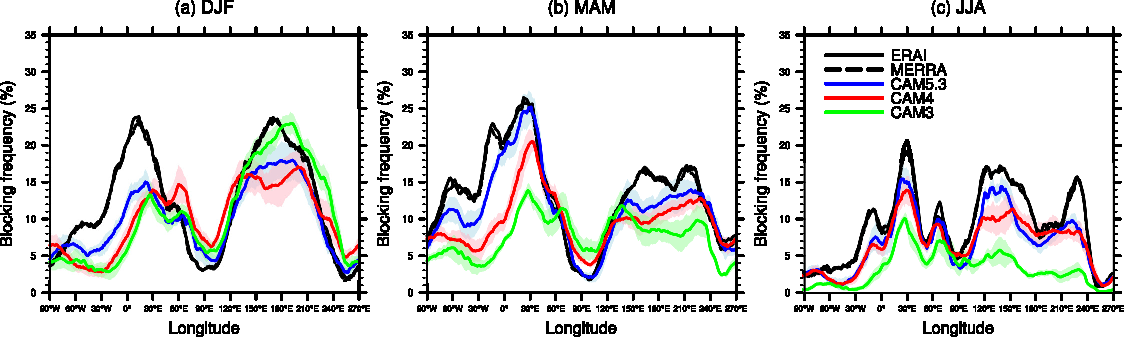
\includegraphics[width=1.0\textwidth,angle=0.]{./figs/f_bfreq.pdf}\\
  \end{center}
  \caption{Seasonal averages of daily blocking frequency (1979-1999) and +/- 1 standard deviation (\%) for ensembles of CAM3, CAM4 and CAM5.3 for (a) Dec/Jan/Feb, (b) Mar/Apr/May, and (c) Jun/Jul/Aug } 
\label{f_bfreq}
\end{figure}

\pagebreak

\begin{figure}[t]
  \begin{center}
    \noindent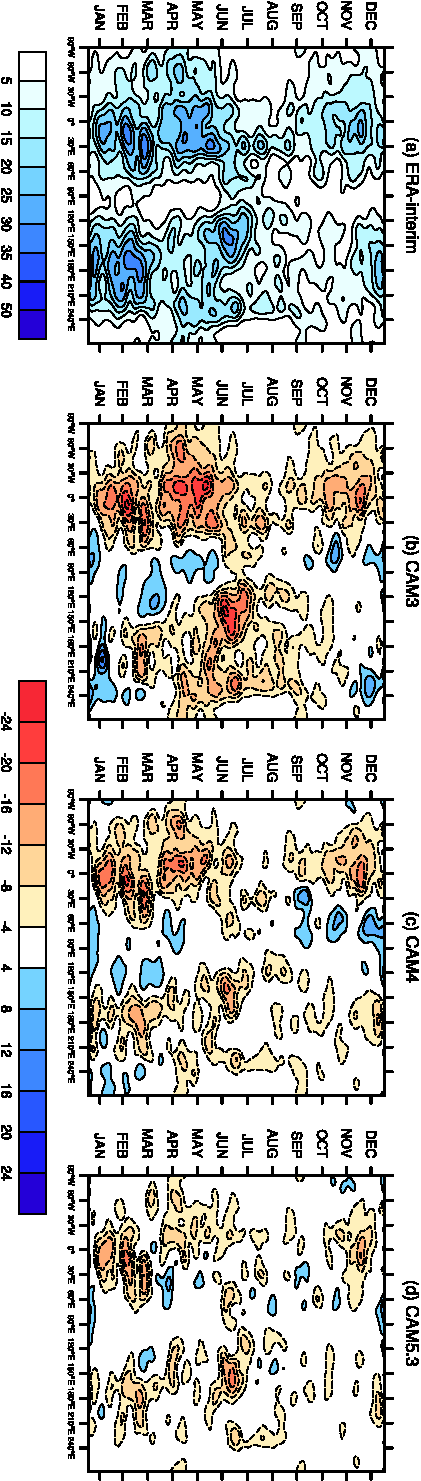
\includegraphics[width=0.3\textwidth,angle=90.]{./figs/f_acycle_block.pdf}\\
  \end{center}
  \caption{Annual cycle of blocking frequency (\%) for (a) ERA-interim and ensemble means of (b) CAM5, (c) CAM4 and (d) CAM3 simulations. Ten passes of a 9x9 local smoother is applied prior to plotting.}
\label{f_acycle_block}
\end{figure}

\pagebreak

\begin{figure}[t]
  \begin{center}
    \noindent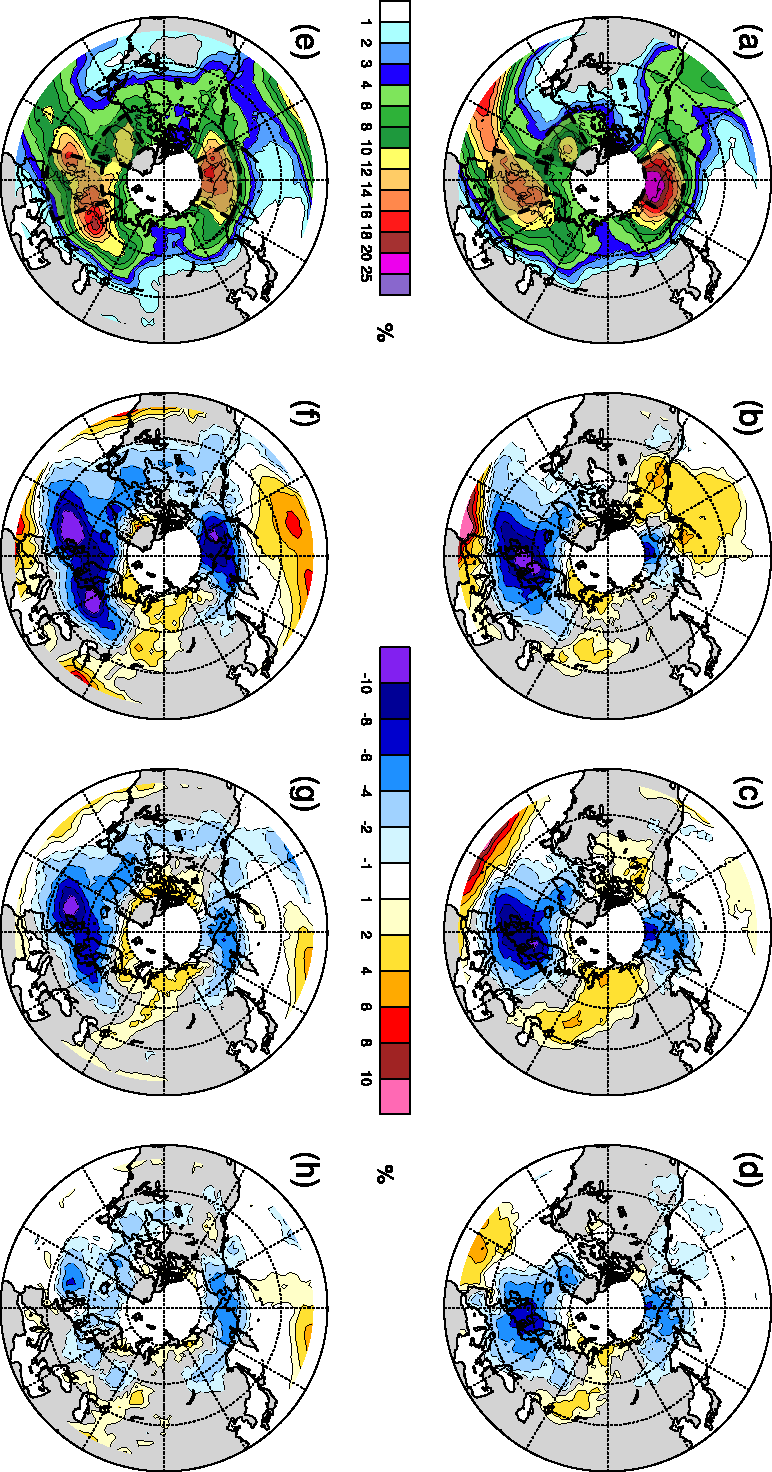
\includegraphics[width=0.55\textwidth,angle=90.]{./figs/f_2d_block.pdf}\\
  \end{center}
  \caption{2-dimensional seasonal average blocking frequency (1979-1999) for Dec/Jan/Feb (top row) and Mar/Apr/May (bottom) row. ERA-interim is shown in (a) and (e) and model biases are shown for CAM3 (b,f), CAM4 (c,g) and CAM5.3 (d,h).} 
\label{f_2d_block}
\end{figure}

\pagebreak

\begin{figure}[t]
  \begin{center}
    \noindent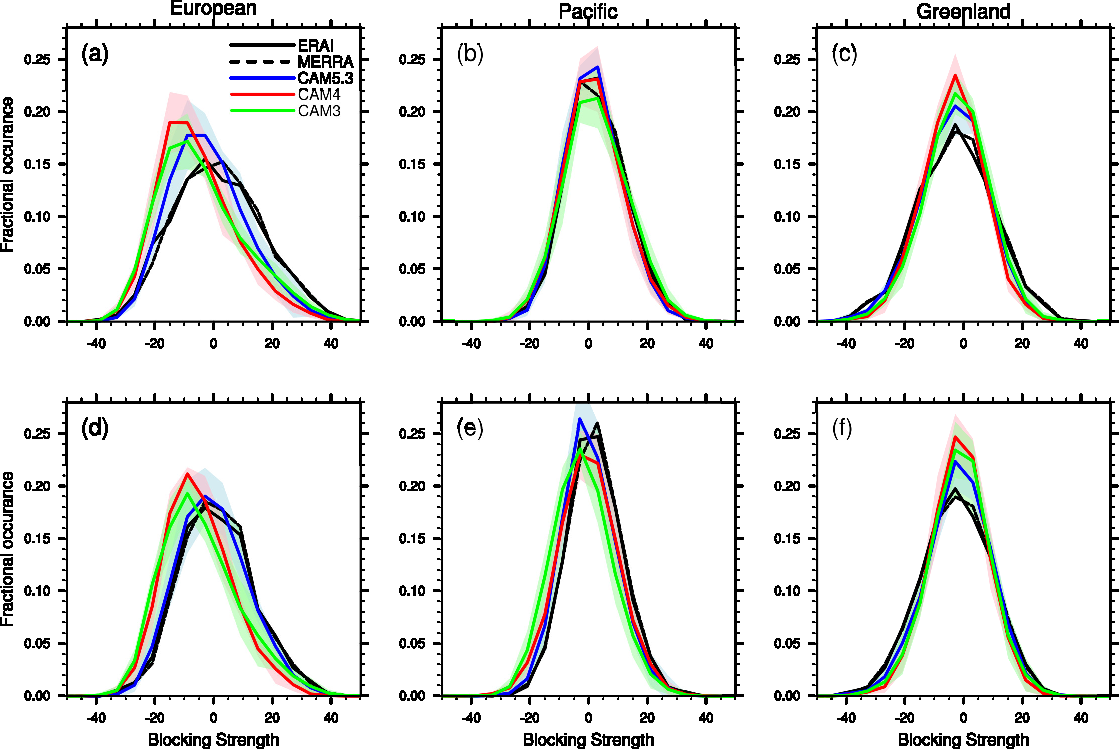
\includegraphics[width=1.0\textwidth,angle=0.]{./figs/f_block_pdf.pdf}\\
  \end{center}
  \caption{PDF of regional daily blocking strength in CAM (1979-1999) for Dec/Jan/Feb (top row) and Mar/Apr/May (bottom) row. Individual regions are defined by the domains in Fig. \ref{f_2d_block}.}
\label{f_block_pdf}
\end{figure}

\pagebreak



\begin{figure}[t]
  \begin{center}
    \noindent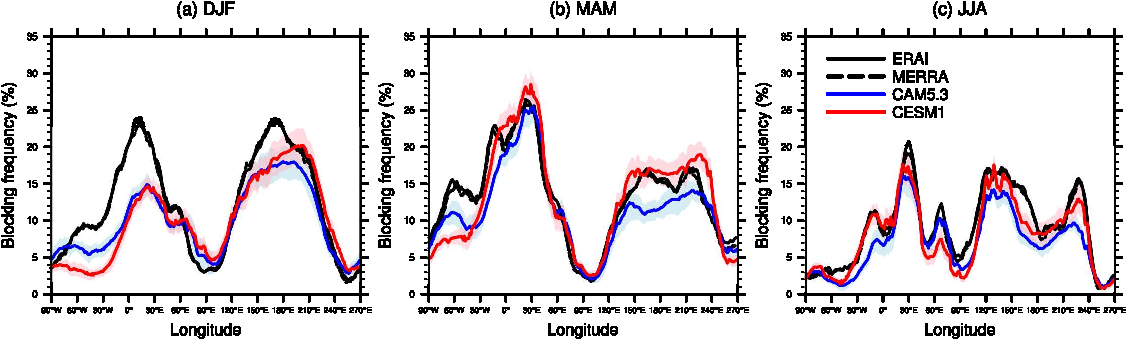
\includegraphics[width=1.0\textwidth,angle=0.]{./figs/f_bfreq_cesm1.pdf}\\
  \end{center}
  \caption{Seasonal averages of daily blocking frequency (1979-1999) and +/- 1 standard deviation (\%) for ensembles of CAM5.3 AMIP and CESM1 fully coupled simulations for (a) Dec/Jan/Feb, (b) Mar/Apr/May, and (c) Jun/Jul/Aug } 
\label{f_bfreq_cesm1}
\end{figure}

\begin{figure}[t]
  \begin{center}
    \noindent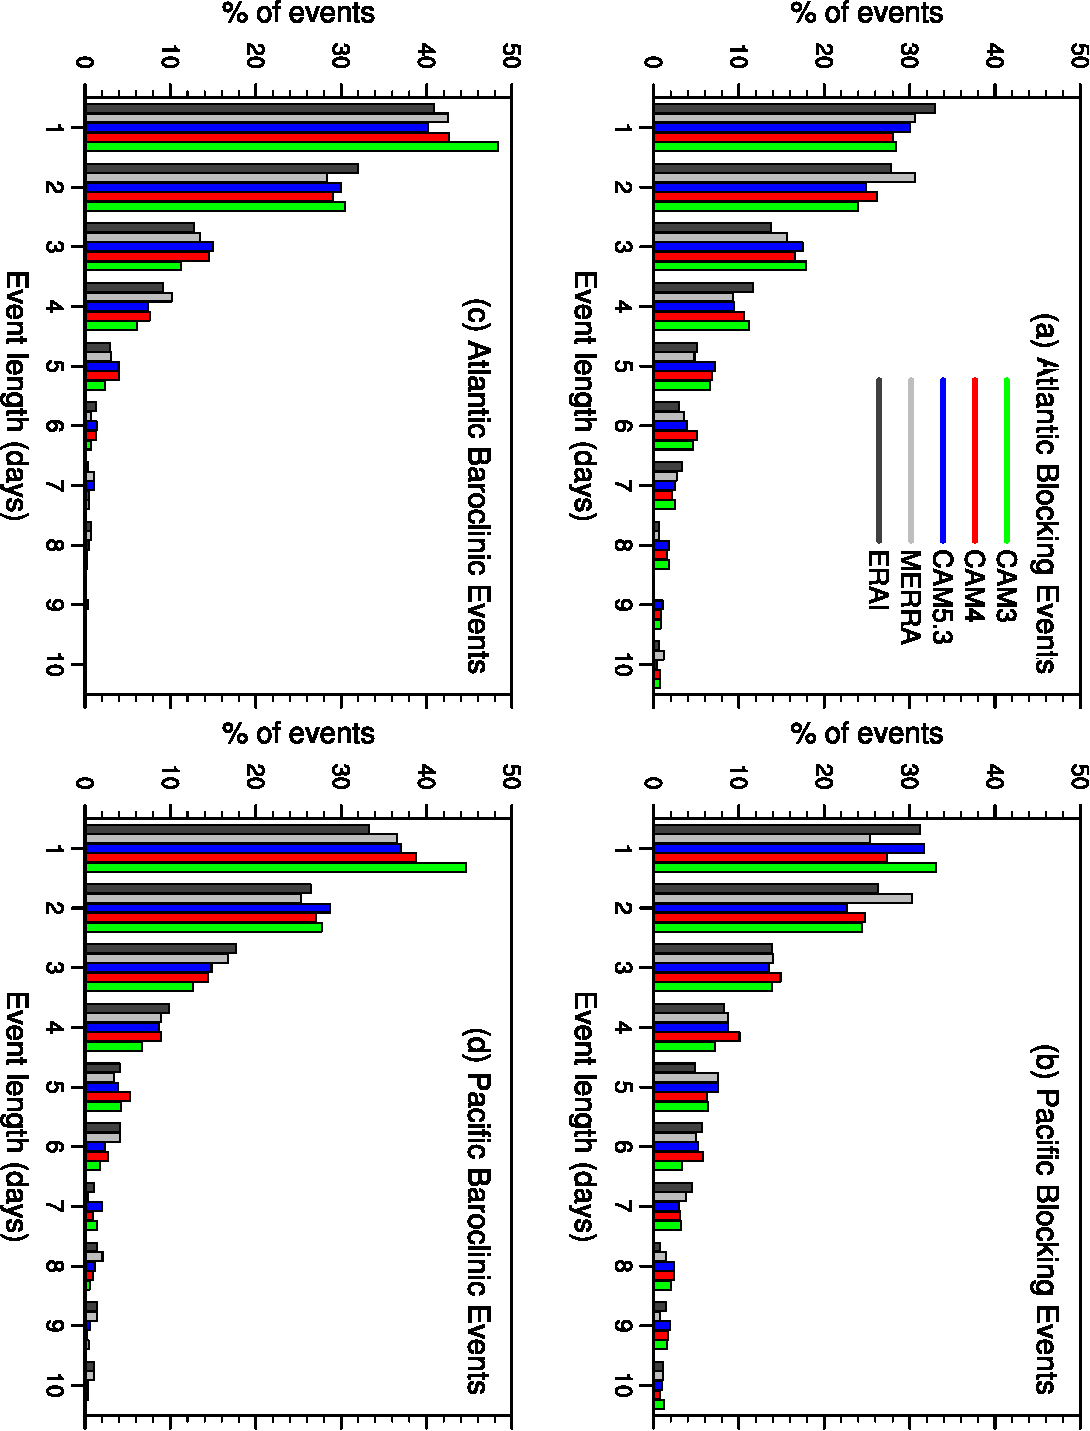
\includegraphics[width=0.75\textwidth,angle=90.]{./figs/f_event_len.pdf}\\
  \end{center}
  \caption{Day-length distributions for baroclinic and blocking events from CAM versions for the Pacific and Atlantic sectors. Events are determined to exist on a particular day when 500-mb height meridional gradient being greater than/less than +/-1.5 times the standard deviation of the blocking index distribution for blocking/barcolinc events.} 
\label{f_event_len}
\end{figure}

\begin{figure}[t]
  \begin{center}
    \noindent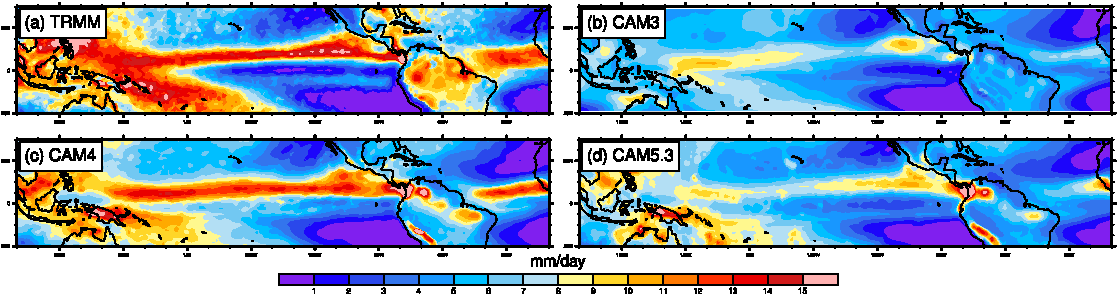
\includegraphics[width=1.0\textwidth,angle=0.]{./figs/f_precip_std.pdf}\\
  \end{center}
  \caption{Standard deviation of precipitation (mm/day) for (a) TRMM (2000-2010), (b) CAM3, (c) CAM4 and (d) CAM5 AMIP simulations (1979-1999)} 
\label{f_precip_std}
\end{figure}

\pagebreak

%%%%%%%%%%%%%%%%%%%%%%%%%%%%%%%%%%%%%%%%%%%%%%%%%%%%%%%%%%%%%%%%%%%%%
% TABLES
%%%%%%%%%%%%%%%%%%%%%%%%%%%%%%%%%%%%%%%%%%%%%%%%%%%%%%%%%%%%%%%%%%%%%
\begin{table}[t]
\caption{Summary details of the CAM and CCSM experiments analyzed using CAM3, CAM4 and intermediate development model versions.}\label{t1}
\begin{center}
\begin{tabular}{cccccrrcrc}
\hline\hline
$Name$ & $Description$ &$SST$ & $Analysis Period$ \\
\hline
CAM3 (T42)       & Spectral low-resolution                         & AMIP     & 1981-2000  \\
CAM3 (T85)       & Spectral high-resolution                        & AMIP     & 1981-2000  \\
CAM3 (2\deg)     & FV low-resolution                               & AMIP     & 1980-1999  \\
CAM3-DIL (2\deg) & FV + CAPE dilution                              & AMIP     & 1980-1999  \\
CAM3-CMT (2\deg) & FV + convective momentum transports             & AMIP     & 1980-1999  \\
CAM3-CONV (2\deg)& FV + convective changes (CMT+DIL)               & AMIP     & 1980-1999  \\
CAM3.5 (2\deg)   & Interim CAM release: \citep{CCSM3.5}            & AMIP     & 1979-2005  \\
                 & FV-CONV+freeze drying+cloud fraction update     &          &            \\
CAM4 (2\deg)     & FV low-resolution                               & AMIP     & 1981-2000  \\
CAM4 (1\deg)     & FV high resolution                              & AMIP     & 1981-2000  \\
\hline
CCSM3 (T85)      & Spectral high-resolution                        & Coupled  & 1970-1999  \\
CCSM4 (2\deg)    & FV low-resolution                               & Coupled  & 1970-1999  \\
CCSM4 (1\deg)    & FV high-resolution                              & Coupled  & 1970-1999  \\
\hline
\end{tabular}
\end{center}
\end{table}
%
\end{document}
